%
% ---------- header -----------------------------------------------------------
%
% project       kaneton
%
% license       kaneton
%
% file          /home/mycure/kaneton/view/book/kaneton/overview.tex
%
% created       julien quintard   [fri jun 15 17:47:20 2007]
% updated       julien quintard   [fri jun 15 17:49:52 2007]
%

%
% ---------- overview ---------------------------------------------------------
%

\chapter{Overview}

In this chapter we will overview the kaneton microkernel design enumerating
the different fundamental managers and their goals.

But first, this chapter will introduce general operating systems
terms as prerequisites for the next chapters of this document.

\newpage

%
% ---------- text -------------------------------------------------------------
%

\section{Generalities}

To understand the kaneton microkernel design and implementation, the reader
must first understand what are the distributed operating systems requirements
and more generally what are distributed systems inherent problems.

As this is not the subject of this document, the reader should probably
look for materials on distributed systems.

Nevertheless we will introduce what is a distributed operating system
just to get a representation of it.

A distributed operating system can be defined through different ways and
the reader should probably find different definitions from different
authors.

For this document, the main goal of a \textbf{distributed operating system}
is to connect users and resources in a transparent, open, and scalable way.

For example, when a user launchs a program, the distributed operating system
decides where to put it, on which machine on the network.

More generally, for any action performed, the distributed operating system
will find out the better way to perform it.

Then, while the processes generally communicate with each other on the same
machine, on a distributed operating system, they also communicate with the
other processes of other machines.

The Figure \ref{figure:overview_distributed-operating-system} illustrates
these communications.

\begin{figure}[h]
  \begin{center}
    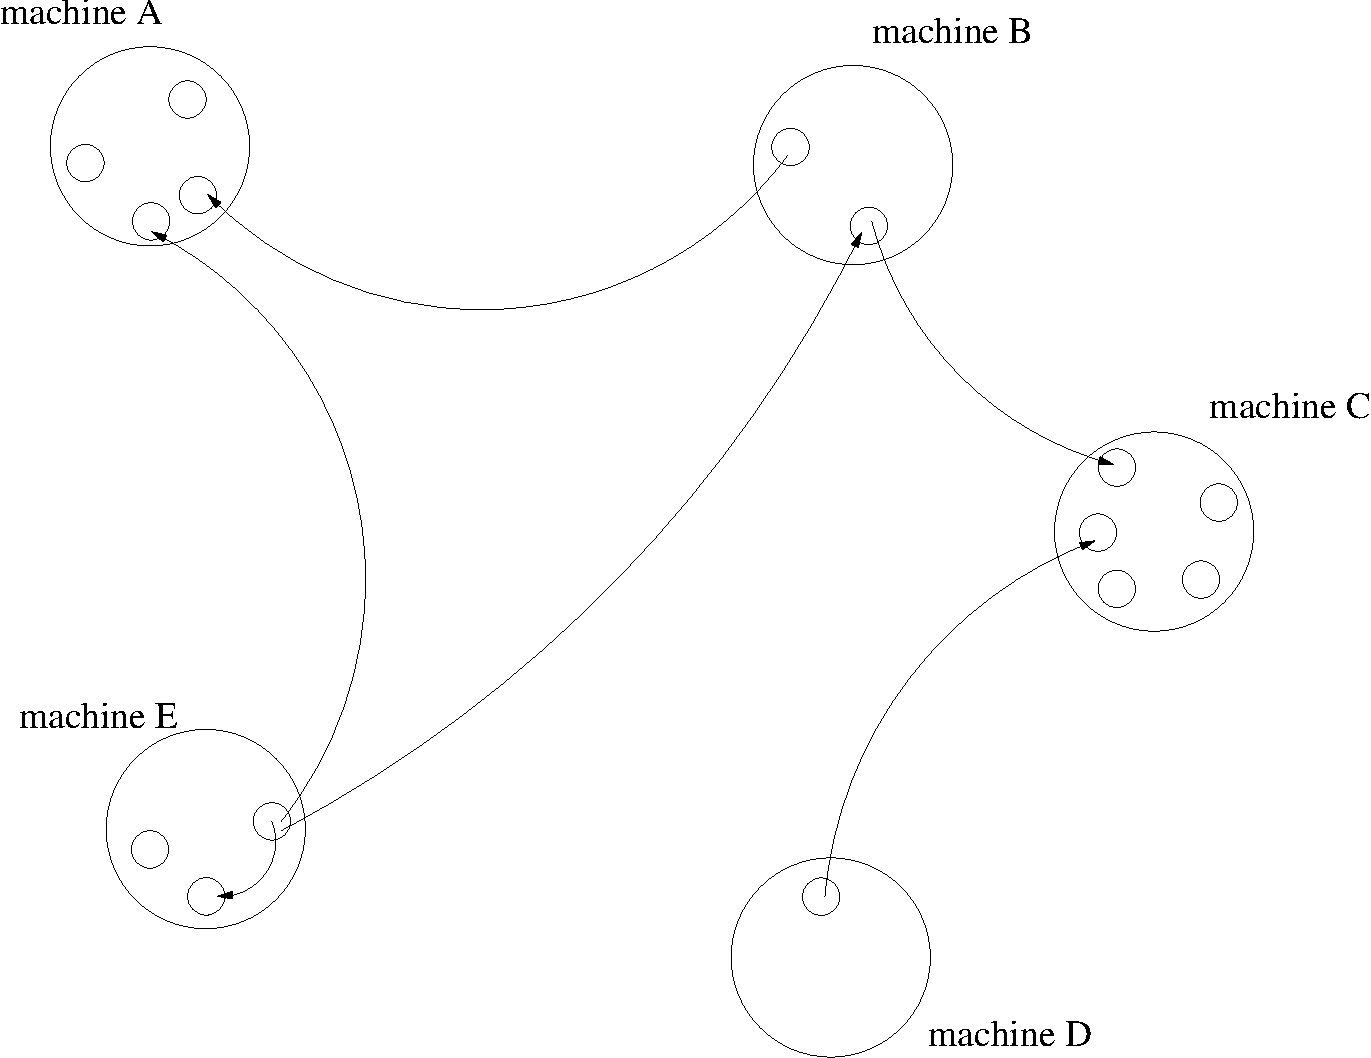
\includegraphics[scale=0.5]{\path/figures/distributed-operating-system.pdf}
    \caption{Communications in a distributed operating system.}
    \label{figure:overview_distributed-operating-system}
  \end{center}
\end{figure}

On the Figure \ref{figure:overview_distributed-operating-system}, the machine
named \textit{E} is running three processes. One is just running some
calculations performing no communication, another is receiving a message
from the latter which is also sending two messages to processes over the
network.

These communications can be simple point-to-point communication for example
between a client and a web server while other can be distributed operating
system specific messages intended to make decisions for example on the
location of a file on the distributed file system.

We saw that machines on a distributed operating system are running processes
which communicate with any other process of any other node. Of course,
every machine needs an operating system to organize the computer resources.

For distributed operating systems requirements, the kernels type used on
each node is by nature microkernel one due to its modular characteristic.

Let's recall what is a microkernel.

A \textbf{microkernel} is a kernel type designed to be modular. Instead
of building a large binary object containing the kernel itself, the drivers,
the file systems etc. microkernels try to be as small as possible,
providing only the fundamental services like managing memory, execution
contexts, communication and input/output. Then the other classical operating
system's services are provided by userland processes with special privileges
called \textbf{servers}.

This very specific design is very interesting for security, maintainability
and extensibility. Moreover, this type of design especially perfectly fit
in distributed operating systems requirements where special processes
communicate with other node's processes to organize the whole distributed
system resources. These processes would be the servers in the microkernel
case while it would be the kernel itself in a monolithic kernel organization.

The Figure \ref{figure:overview_microkernel} illustrates a microkernel
view with different layers.

\begin{figure}[h]
  \begin{center}
    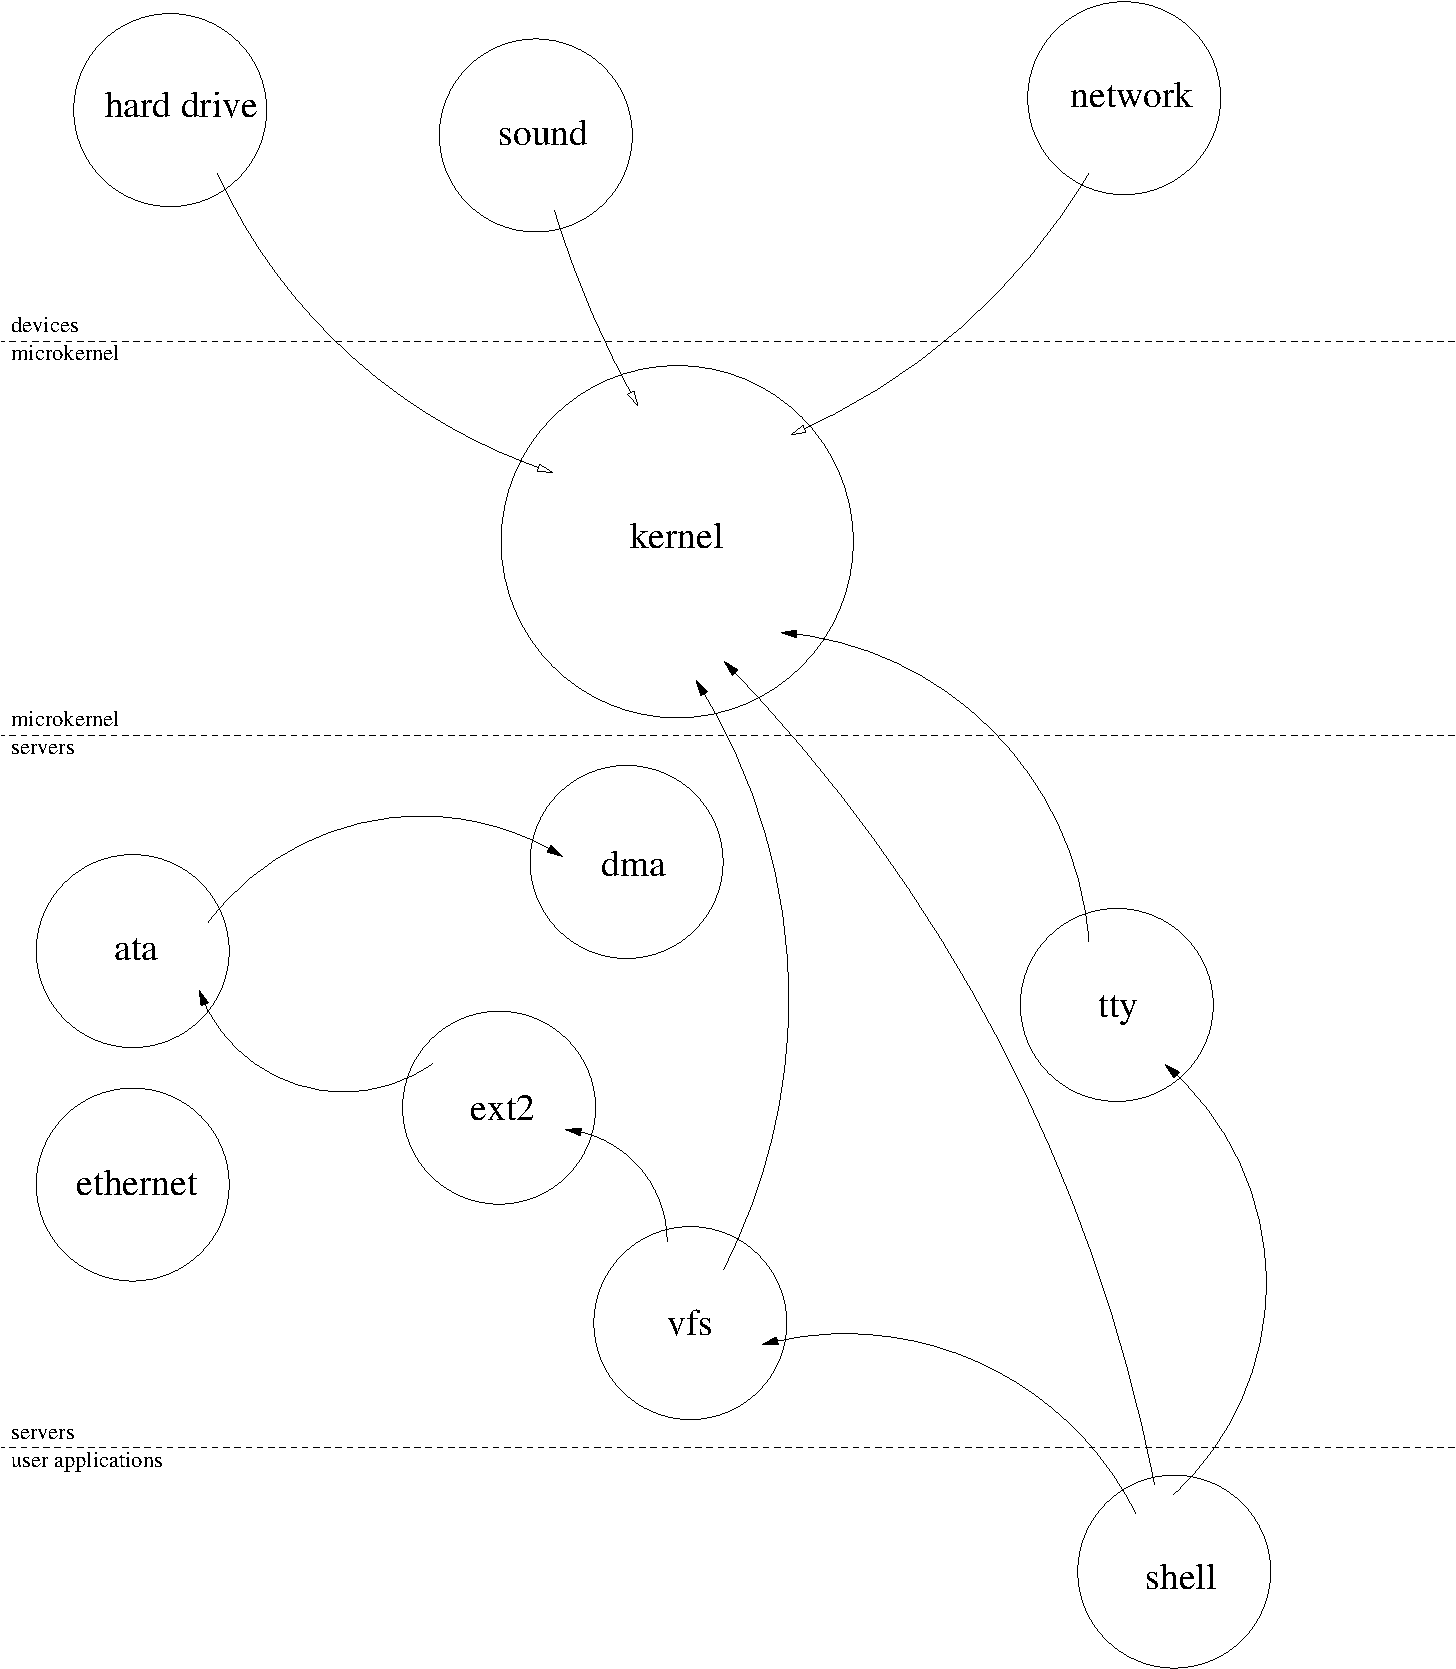
\includegraphics[scale=0.5]{\path/figures/microkernel-behaviour.pdf}
    \caption{Communications in a microkernel's hierarchy.}
    \label{figure:overview_microkernel}
  \end{center}
\end{figure}

The whole microkernel design is based on the client-server communication
model where clients ask servers to perform a specific task.

For example to print some text to the screen a user program has to
ask the \textit{tty} server to do so because the user program itself does
not have the permission to do it.

To avoid complications and deadlocks the microkernels follow a fundamental
rule which restrict communication from clients only to more or equal
privileged tasks.

On the Figure \ref{figure:overview_microkernel}, the \textit{vfs} server can
ask the \textit{ata} server and the \textit{kernel} to peform a task but
the kernel cannot ask a less privileged server to do something.

Some kernels break this rule for specific reasons. More precisly,
when the kernel itself stop its execution context to run a less
privileged process, the kernel does what we call an \textbf{upcall}.

Upcalls must be avoided because its means the design is deficient.

\section{kaneton}

Assuming the reader is now aware of kernel generalities and more
precisly of microkernel designs and their close relation with
distributed operating systems we will try to establish a link
between common kernel functionalities and kaneton via the
kaneton nomenclature.

As said before the kaneton microkernel is only the core of an
operating system. Main tasks like hardware device drivers or
user services are implemented as servers. So the microkernel
only has a few functionalities to provide:

\begin{itemize}
  \item
    Memory Management.
  \item
    Execution Contexts Management.
  \item
    Communication Management.
  \item
    Inputs/Outputs Management.
\end{itemize}

The kaneton microkernel itself was designed to be heavily
modular. Indeed, the kaneton source code is divided into managers
each manager taking care of performing tasks on specific kaneton
objects.

We will now describe each microkernel functionality taking care of
enumerating the kaneton managers involved in.

%
% memory management
%

\subsection{Memory Management}

The memory management consists in providing primitives to perform
low-level tasks like reserving, releasing, modifying properties on
physical and virtual memories.

Most kernels divide the memory management into two distinctive
parts, one for the physical memory and the other for the virtual one.

Then, the physical memory manager knows what are the physical memory
ranges reserved and used and what are the ones which are not. This
manager so just keeps an internal data structure describing the
physical memory state.

In practice its is a little bit more complex than that.

The virtual memory manager manages the virtual memory of every
processes establishing mappings between virtual and physical memory
ranges.

In kaneton, there are three managers involved in the memory management.

The first, called the \textbf{address space} manager manages address
space object. An address space object contains the list of addressable
memory locations including a list of physical memory locations and
a list of virtual memory locations.

Each task has its own address space so this manager will be heavily
used the task manager.

The second manager involved in the memory management is called the
\textbf{segment manager}. This manager manages the physical memory
as other kernel's physical memory manager do. Indeed, its role
is to provide access to low-level functionalities dealing with
physical memory to reserve, release etc. memory.

This manager is the most important of the three ones.

The latter is called the \textbf{region manager} and is equivalent
to the virtual memory manager of other kernels. This manager so just
manages the mappings between virtual and physical memory locations.

%
% process management
%

\subsection{Execution Contexts Management}

The execution contexts management consits in providing a complete
interface to create, extend, destroy etc. execution contexts.

In kaneton, there are two managers involved in execution contexts
management.

The first one, called \textbf{task manager} manages the task object.

A task, in kaneton terms, is exactly an execution context. Indeed,
a task object is composed of an address space and one or more
threads.

The task manager so provide everything necessary to create, destroy
and control tasks.

The second manager involved in execution contexts management is called
\textbf{thread manager} since its role is to manage threads.

In kaneton, the active entity, the scheduled entity is the thread. The
task object is in fact just an abstraction describing the entire execution
context.

The thread manager permit to add, remove, start, stop etc. threads
of the task them belong to.

Notice that another manager exists, called the \textbf{scheduler} but
its role is to schedule the execution contexts and not to really to
manage them.

%
% communication
%

\subsection{Communication Management}

We know which manager deals with process and memory management.

The communication is an important issue since very first microkernels
had poor performances due to bad communication design and implementation.

The kaneton \textbf{message manager} is very important since its
role is to provide a powerful interface to communication including
a very large panel of communication types.

%
% inputs/outputs
%

\subsection{Inputs/Outputs Management}

The inputs and outputs are internally managed in monolithic
kernels while microkernel generally abstract them to a more high-level
object.

In kaneton, every input/output is abstracted in an event.

Then, the \textbf{event manager} manages the events in a very simple way.

%
% internal view
%

\subsection{View}

To conclude, the Figure \ref{figure:overview_kaneton} illustrates the core's
internal organization with its multiple managers.

\begin{figure}[h]
  \begin{center}
    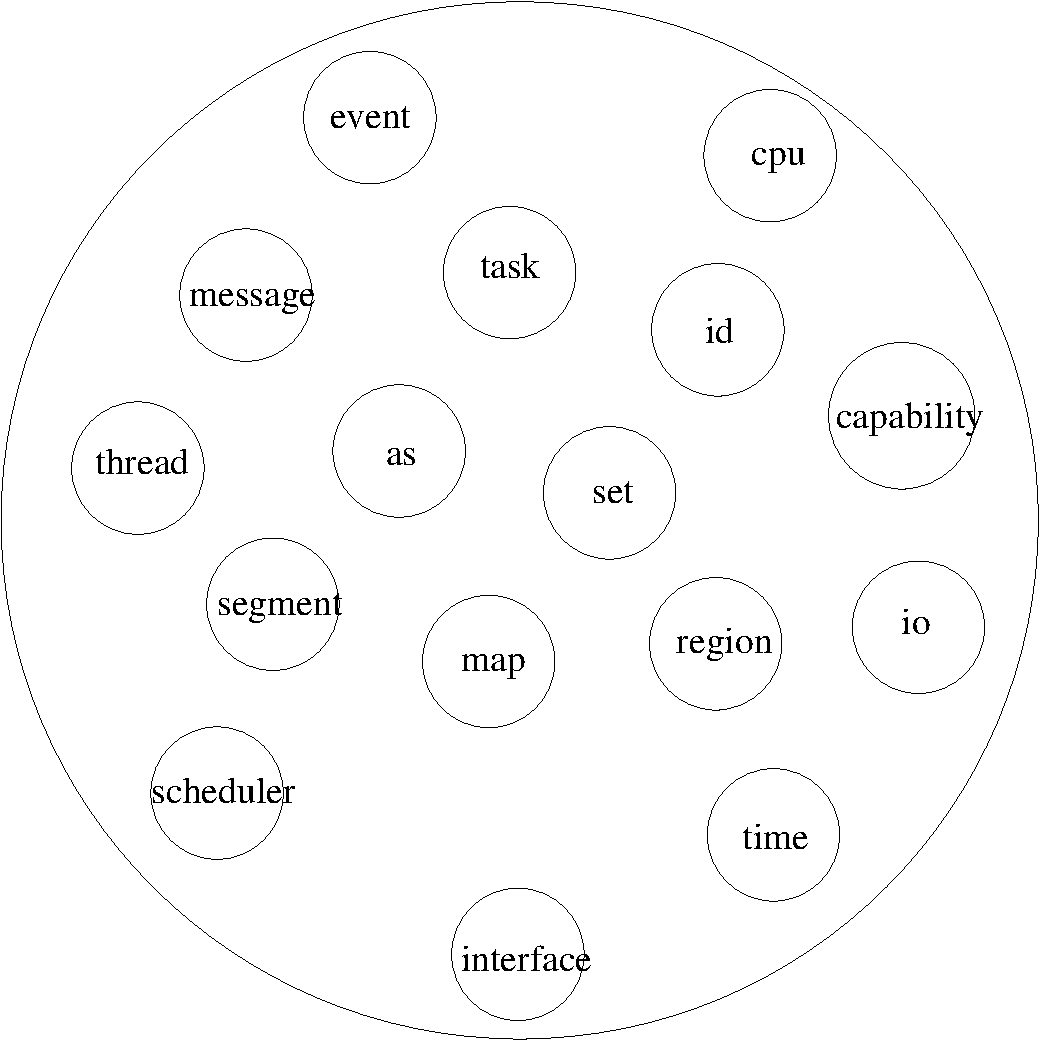
\includegraphics[scale=0.5]{\path/figures/kaneton-managers.pdf}
    \caption{kaneton internal managers.}
    \label{figure:overview_kaneton}
  \end{center}
\end{figure}

XXX a retoucher completement
